\documentclass[aspectratio=169]{beamer} %43 169
\usetheme{CambridgeUS}
\setbeamertemplate{section in toc}[sections numbered]
\setbeamertemplate{subsection in toc}[subsections numbered]
\setbeamertemplate{headline}{}

% elementary packages:
\usepackage{graphicx}
\usepackage[latin1]{inputenc}
\usepackage[T1]{fontenc}
\usepackage[english]{babel}
\usepackage{listings}
\usepackage{xcolor}
\usepackage{eso-pic}
\usepackage{mathrsfs}
\usepackage{url}
\usepackage{amssymb}
\usepackage{amsmath}
\usepackage{multirow}
\usepackage{hyperref}
\usepackage{amsmath} 
\usepackage{verbatim} %for comment environment

% additional packages
\usepackage{bbm}
\usepackage[export]{adjustbox}
\usepackage{booktabs}
\usepackage{algorithm} %for pseudo code
\usepackage[noend]{algpseudocode} %for pseudo code
\usepackage{lmodern} %font for algorithm package

% Define the title.  
\title[Causal KNN]{Causal KNN}
\subtitle{}
\author{Seminar Applied Predictive Analytics}
\institute[]{Maximilian Kricke\\Tim Peschenz\\ \vspace{0.5cm} Chair of Information Systems\\Humboldt Universit\"at zu Berlin}
\date{27.06.2019}


%margins
\setbeamersize{text margin left=0.8cm,text margin right=0.8cm} 

%arg min in formulars
\newcommand{\argmin}[1]{\underset{#1}{\operatorname{arg}\,\operatorname{min}}\;}

% start pdf file in full screen mode
\hypersetup{pdfpagemode=FullScreen}


%Start of the document
\begin{document}

\setbeamertemplate{itemize items}[circle]

% title page
\frame[plain]{
\titlepage
\centering{

\includegraphics[width=2cm]{logo}
}
}

% Outline
\frame{
\frametitle{Outline}
\tableofcontents
}

\section{Motivation}

\subsection{Course Framework of our Topic}

\frame{
\frametitle{Course Framework}
\centering

\includegraphics[width=10cm]{Objects/course_framework.pdf}
\begin{itemize}
\item Paper: "Heterogeneous Treatment Effects and Optimal Targeting Policy Evaluation" (Hitsch and Misra 2018)
\item Potential Outcomes Framework and the Fundamental Problem of Causal Inference:\\
  \textit{We never observe the individual treatment effect but only the outcome corresponding to the assigned treatment.}
\end{itemize}
}

\frame{
\frametitle{Course Framework of our Topic}
\begin{itemize}

\item Method to somehow overcome this fundamental problem
\item General parameter tuning technique for uplift models
\item Applicable tool to evaluate different targeting policies using only one data set
\end{itemize}
}

\subsection{Business Framework}
\frame{
\frametitle{Business Framework}
\begin{itemize}
\item\textbf{Imagine you run a marketing campaign}
\item How do you measure if a campaign was successful or not?
\item To optimize a marketing campaign, you should decide based on customer level:
\begin{itemize}
\item A customer should be targeted if the individual profit contribution is greater than the targeting cost for this individual.\\
\end{itemize}
\vspace{0.5cm} 
It is shown that the CATE on an individual basis is sufficient to construct an optimal targeting policy.\\
\vspace{0.5cm}
\textit{But how can we measure the (unobservable) individual CATE?}
\end{itemize}
}

\subsection{Measuring the Individual CATE}

\frame{
\frametitle{Measuring the individual CATE}
\begin{itemize}
\item[]
We need to make three assumptions to the data:
\begin{itemize}
\item Unconfoundedness: $Y_i(0), Y_i(1) \perp W_i | X_i$ (random assignment of the treatment within each subgroup of the population with identical features $X_i = x$)
\item No overlap: $0<e(x)<1$
\item Stable Unit Treatment Value Assumption (SUTVA): No social interactions or equilibrium effects
\end{itemize}

If these assumptions are satisfied, we can compute the CATE via:

\begin{center}
$\tau(x) = \mathbb{E}[Y_i|X_i,W_i = 1] - \mathbb{E}[Y_i|X_i,W_i = 0]$
\end{center}

\vspace{0.5cm}
Hence we are calculating the mean difference between the outcomes of treated and untreated units with identical features. 
\vspace{0.5cm}

\textit{But do we even have individuals with the same features?}
\end{itemize}
}


\section{Causal KNN}
\subsection{Causal KNN Algorithm}

\frame{
\frametitle{Outline}
\tableofcontents[currentsection]
}


\frame{
\frametitle{The Causal KNN Approach}

\begin{itemize}
%\item CATE represents expected causal effect of being targeted versus not being targeted for a customer with observed features $X_i = x$ (Hitsch and Misra, 2018)
\item direct estimation of the conditional average treatment effect $\hat{\tau}_i$ for all observations i, by comparing the mean outcome of the nearest neighbours 
\item selecting nearest neighbours based on the covariates $X_i$ using the euclidian distance measure 
\item compare outcomes $Y$ of k treated $Y(w=1)$ and k untreated $Y(w=0)$ nearest neighbours of unit i, to derive an estimation $\hat{\tau}_i$ of the conditional average treatment effect $\tau_i$
\end{itemize}

\vspace{0.5cm}

\centering{
$\hat{\tau}_K(x)= \frac{1}{K} \sum\limits_{i \in \mathcal{N}_K(x,1)} Y_i - \frac{1}{K}  \sum\limits_{i \in \mathcal{N}_K(x,0)} Y_i$

}
}

\frame{
\frametitle{The Causal KNN Approach}
\begin{center}
\scalebox{0.75}{
    \begin{minipage}{1.25\linewidth}
\begin{algorithm}[H]
\caption{Causal KNN Algorithm}
\begin{algorithmic}

\Procedure{CausalKNN}{$k, y, w, x$}
	\State Input:
    \State \hspace{0.5cm} $k \rightarrow$ number of nearest neighbours
    \State \hspace{0.5cm} $y \rightarrow$ vector with outcome values
    \State \hspace{0.5cm} $w \rightarrow$ vector with treatment status
    \State \hspace{0.5cm} $x \rightarrow$ matrix with covariates
    \vspace{0.5cm}
    \State \textbf{Begin}
    \State 1. select nearest neighbours for each observation i based on the covariates x
    \State 2. separate k treated $(w_i = 1)$ and k untreated $(w_i = 0)$ nearest neighbours
     \For {each observation i}
        \State calculate mean of $y_k(w = 1)$ and $y_k(w = 0)$
        \State $uplift_i =$ mean of $y_k(w = 1)$ - mean of $y_k(w = 0)$
      \EndFor
      \State \textbf{End}
\EndProcedure  


\end{algorithmic}
\end{algorithm}
\end{minipage}
}
\end{center}
}



\subsection{Causal KNN Example}
\frame{
\frametitle{Causal KNN Example}

\begin{itemize}
\item k value has to be set in advance
\item example table with necessary input information
\end{itemize}
\begin{table}[]
\begin{tabular}{@{}lllllll@{}}
\toprule
\textbf{i} & \textbf{W} & \textbf{Y} & \textbf{$X_1$} & \textbf{$X_2$}     & $\cdots$    & $X_m$  \\ \midrule
1          & 1          & 10         & $x_{11}$         & $x_{12}$         & $\cdots$    & $x_{1m}$ \\
2          & 1          & 20         & $x_{21}$         & $x_{22}$         & $\cdots$    & $x_{2m}$ \\
3          & 0          & 25         & $x_{31}$         & $x_{32}$         & $\cdots$    & $x_{3m}$ \\
4          & 0          & 10         & $x_{41}$         & $x_{42}$         & $\cdots$    & $x_{4m}$ \\
\vdots     & \vdots     & \vdots     & \vdots           & \vdots           & $\ddots$    & \vdots \\
n          & 1          & 30         & $x_{n1}$         & $x_{n2}$         & $\cdots$    & $x_{nm}$ \\ \bottomrule
\end{tabular}
\end{table}

\vspace{0.3cm}

\centering{
$\hat{\tau}_K(x)= \frac{1}{K} \sum\limits_{i \in \mathcal{N}_K(x,1)} Y_i - \frac{1}{K}  \sum\limits_{i \in \mathcal{N}_K(x,0)} Y_i$

}

\vspace{0.3cm}

\begin{itemize}
\item[]
\textit{But how should we decide on the optimal value of k?}
\end{itemize}
}

\section{Transformed Outcome}
\frame{
\frametitle{Outline}
\tableofcontents[currentsection]
}

\frame{
\frametitle{Transformed Outcome}
\begin{itemize}
\item \textbf{Idea}:\\ Define a proxy for the true CATE $\tau(X_i)$ to apply the MSE-Criterion: $\mathbb{E}[(\tau(X_i)-\hat{\tau}_K(X_i))^2]$
\item Define the transformed outcome as:
\begin{align}
Y_i^*=W_i\cdot\frac{Y_i(1)}{e(X_i)}-(1-W_i)\cdot\frac{Y_i(0)}{1-e(X_i)}
\end{align}
\item We can rewrite this to:
\begin{align*}
Y_i^*=\frac{W_i-e(X_i)}{e(X_i)(1-e(X_i))}Y_i^{obs}
\end{align*}
 to observe it for all units i.
\end{itemize}
}

\subsection{Justification}
\frame{
\frametitle{Justification for the Transformed Outcome: }
\begin{align*}
Y_i^*&=W_i\cdot\frac{Y_i(1)}{e(X_i)}-(1-W_i)\cdot\frac{Y_i(0)}{1-e(X_i)}\quad|\quad\mathbb{E}[\cdot|X_i=x]\\
&=\mathbb{E}[W_i|X_i=x]\cdot\frac{\mathbb{E}[Y_i(1)|X_i=x]}{e(X_i)}-\mathbb{E}[1-W_i|X_i=x]\cdot\frac{\mathbb{E}[Y_i(0)|X_i=x]}{1-e(X_i)}\\
&=e(X_i)\cdot\frac{\mathbb{E}[Y_i(1)|X_i=x]}{e(X_i)}-(1-e(X_i))\cdot\frac{\mathbb{E}[Y_i(0)|X_i=x]}{1-e(X_i)}\\
&=\mathbb{E}[Y_i(1)|X_i=x]-\mathbb{E}[Y_i(0)|X_i=x]\quad|\quad\textbf{Unconfoundedness}\\
&=\mathbb{E}[Y_i(1)-Y_i(0)|X_i=x]\\
&=\tau(X)
\end{align*}
Hence, the transformed outcome is an unbiased estimate of the CATE and can therefore be used as the desired proxy.
}

\subsection{Transformed Outcome Loss}
\frame{
\frametitle{Transformed Outcome Loss}
\begin{itemize}
\item Now we can define the transformed outcome loss as: 
\begin{align*}
\mathbb{E}[(Y^*_i-\hat{\tau}_K(X_i))^2]
\end{align*}
\item The value for k that minimizes the outcome loss is optimal for our estimation
\end{itemize}
\begin{align}
\arg\min_{K} = \mathbb{E}[(Y^*_i-\hat{\tau}_K(X_i))^2]
\end{align}
%\argmin{K}
}

%argmin_k = \mathbb{E}[(Y^*_i-\hat{\tau}_K(X_i))^2]

\begin{comment}
\subsection{Parameter Tuning}

\frame{
\frametitle{Parameter Tuning using the Transformed Outcome Loss}
\begin{itemize}
\item choosing parameter K to minimize expected transformed outcome loss similar to minimize expected mean squared error (MSE)
\item The following plot shows alternative realizations of the transformed outcome loss for different values of k
\end{itemize}
}
\end{comment}


\begin{comment}
\frame{
\frametitle{Parameter Tuning using the Transformed Outcome Loss (cont.)}
\centering
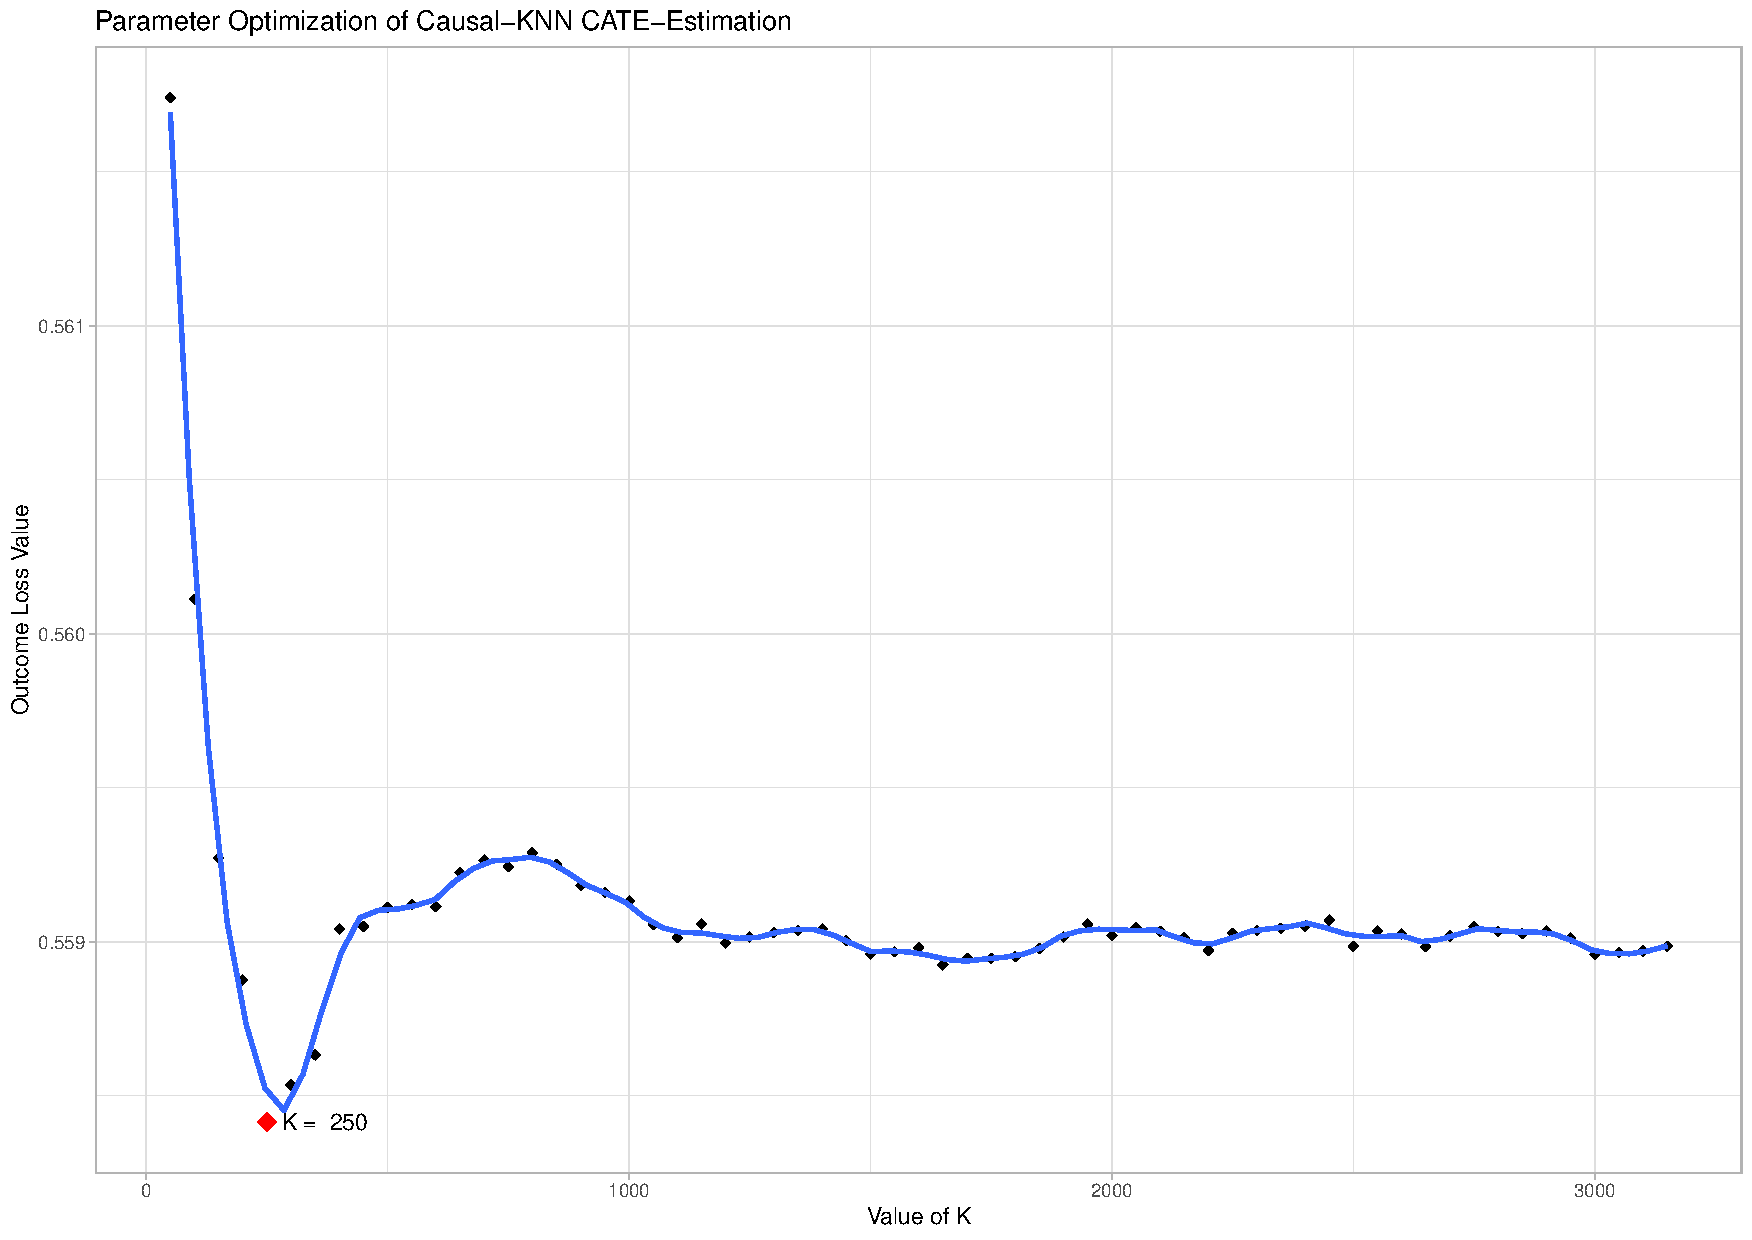
\includegraphics[width=10cm]{Objects/param_tuning.pdf}
}
\end{comment}


\section{Application Part}
\frame{
\frametitle{Outline}
\tableofcontents[currentsection]
}

\frame{
\frametitle{Application: Data Presentation}
\begin{table}[ht]
\resizebox{1\textwidth}{!}{
\centering
\begin{tabular}{rrlrrrlrllrrr}
  \hline
 & recency & history\_segment & history & mens & womens & zip\_code & newbie & channel & segment & visit & conversion & spend \\ 
  \hline
1 & 10.00 & 2) \$100 - \$200 & 142.44 & 1 & 0 & Suburban & 0 & Phone & Womens E-Mail & 0 & 0 & 0.00 \\ 
  2 & 6.00 & 3) \$200 - \$350 & 329.08 & 1 & 1 & Rural & 1 & Web & No E-Mail & 0 & 0 & 0.00 \\ 
  3 & 7.00 & 2) \$100 - \$200 & 180.65 & 0 & 1 & Suburban & 1 & Web & Womens E-Mail & 0 & 0 & 0.00 \\ 
  4 & 9.00 & 5) \$500 - \$750 & 675.83 & 1 & 0 & Rural & 1 & Web & Mens E-Mail & 0 & 0 & 0.00 \\ 
  5 & 2.00 & 1) \$0 - \$100 & 45.34 & 1 & 0 & Urban & 0 & Web & Womens E-Mail & 0 & 0 & 0.00 \\ 
  6 & 6.00 & 2) \$100 - \$200 & 134.83 & 0 & 1 & Suburban & 0 & Phone & Womens E-Mail & 1 & 0 & 0.00 \\ 
   \hline
\end{tabular}}
\end{table}
\begin{itemize}
\item Data base that captures 64.000 customer transactions
\item Treatment Variable "segment"
\item Outcome variables: "visit", "conversion" (binary) and "spend" (numeric) 
\end{itemize}
}


\frame{
\frametitle{Application: Process}
\begin{itemize}
\item Calculate individual CATE for all observations in the data using Causal KNN
\item Select optimal K value by finding the minimal transformed outcome loss value
\item choosing parameter K to minimize expected transformed outcome loss similar to minimize expected mean squared error (MSE)
\end{itemize}

\vspace{0.3cm}

\begin{itemize}
\item parameter tuning for different Uplift Modeling Technique
\item Causal Tree Model Tuning
\end{itemize}
}

\begin{comment}
\frame{
\frametitle{Causal Tree - Parameter Tuning}
\centering
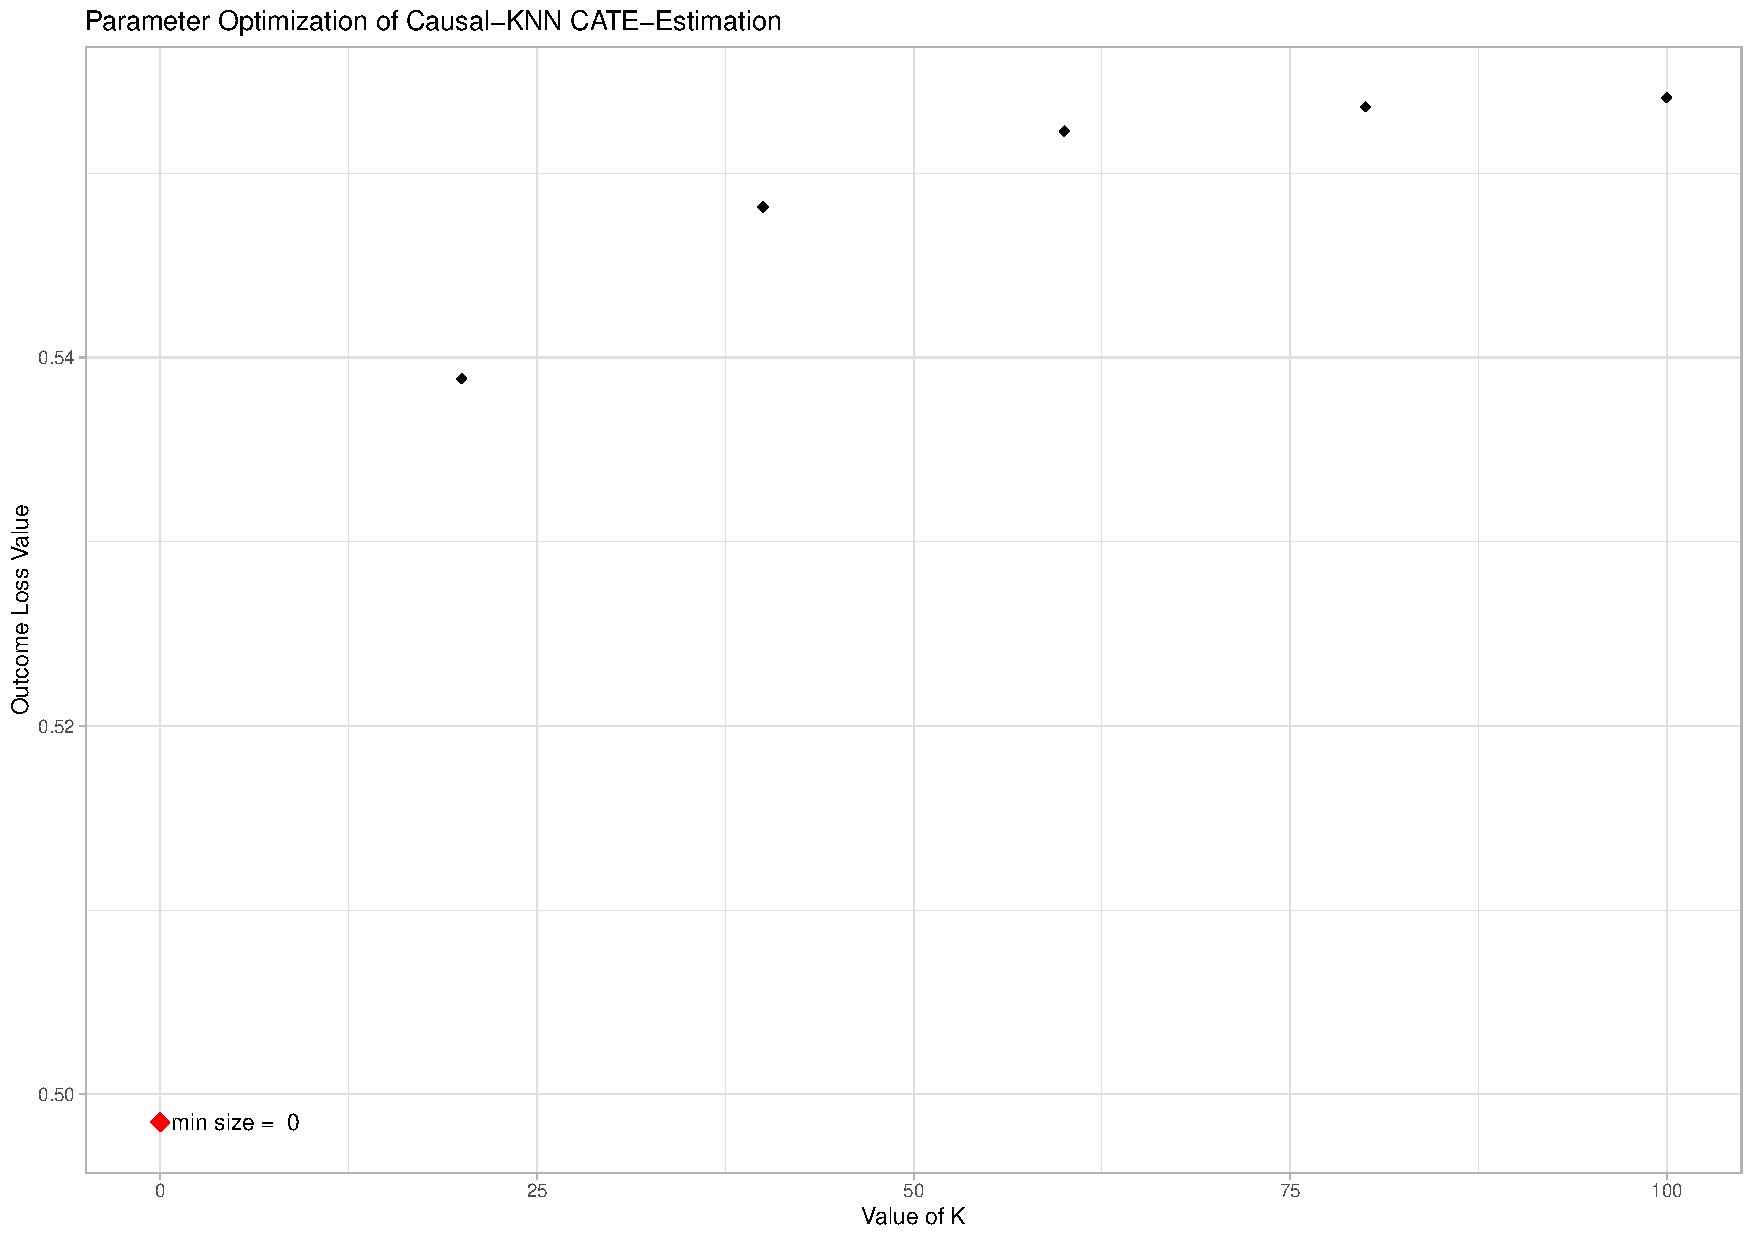
\includegraphics[width=10cm]{Objects/param_tuning_causal_tree.pdf}
}
\end{comment}


\frame{
\frametitle{Application: Results}
\centering
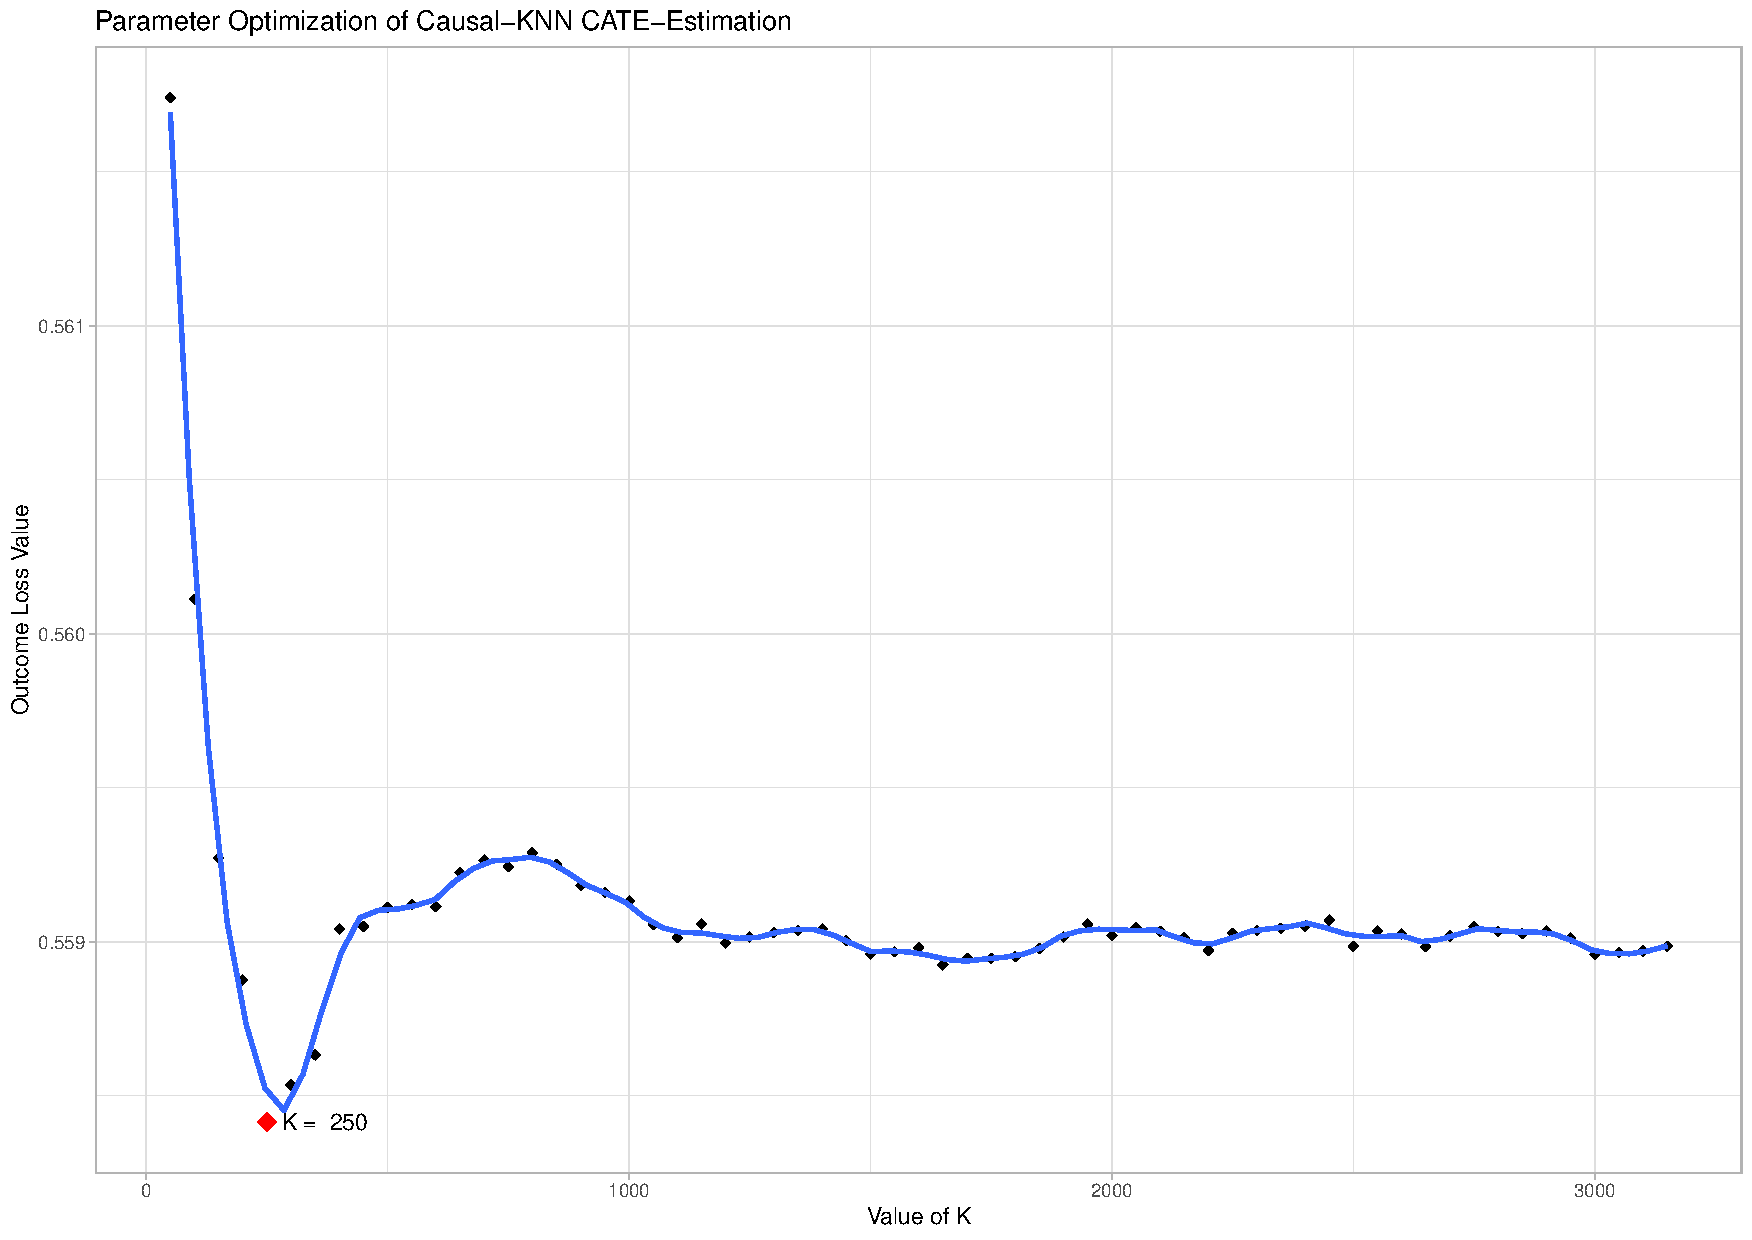
\includegraphics[width=10cm]{Objects/param_tuning.pdf}
}

\frame{
\frametitle{Application: Results}
Outcome Variable: Visit (binary)
\begin{itemize}
\item ATE = 0.05497
\item ATT = 0.05513
\end{itemize}
\vspace{0.2cm}
\centering{
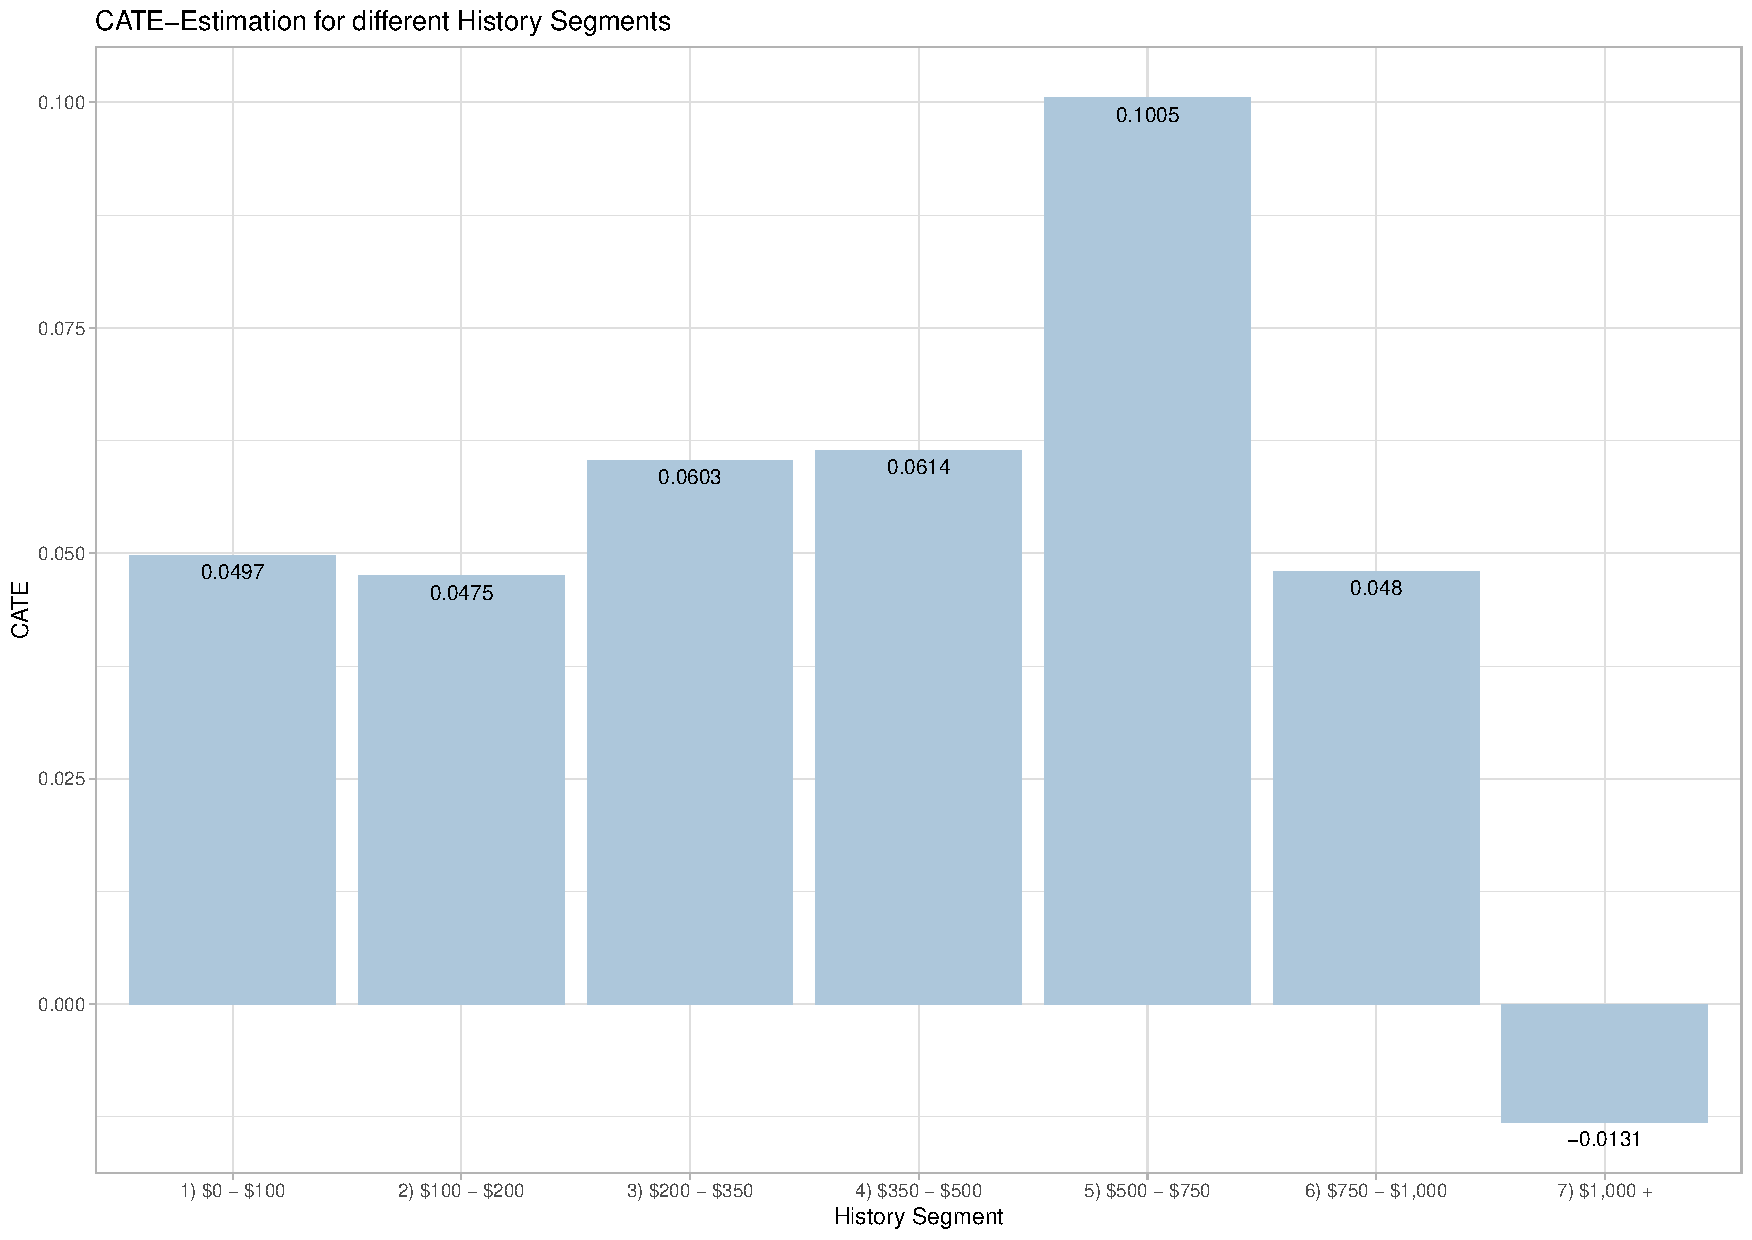
\includegraphics[width=7cm]{Objects/hist_seg_visit.pdf} \hspace{0.2cm}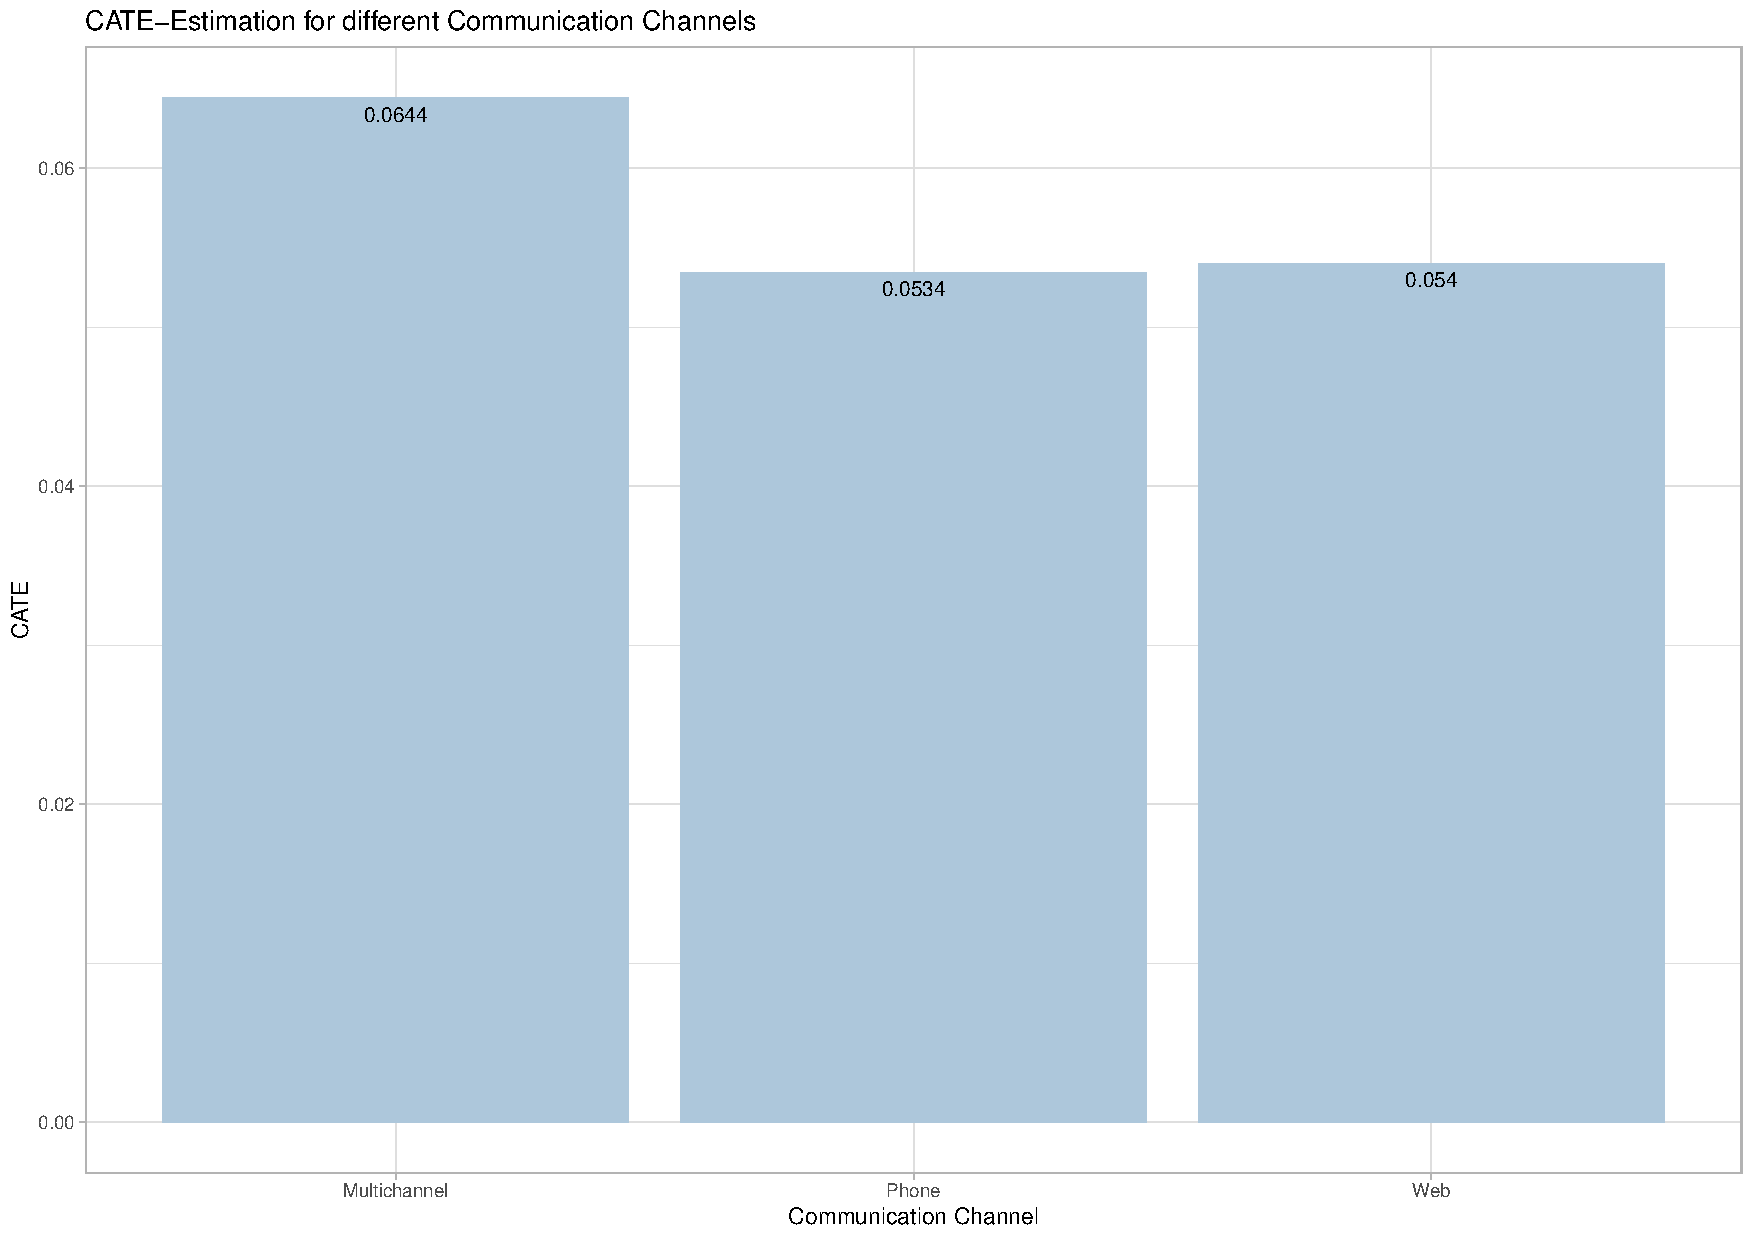
\includegraphics[width=7cm]{Objects/channel_visit.pdf}
}
}

\frame{
\frametitle{Application: Results}
\centering
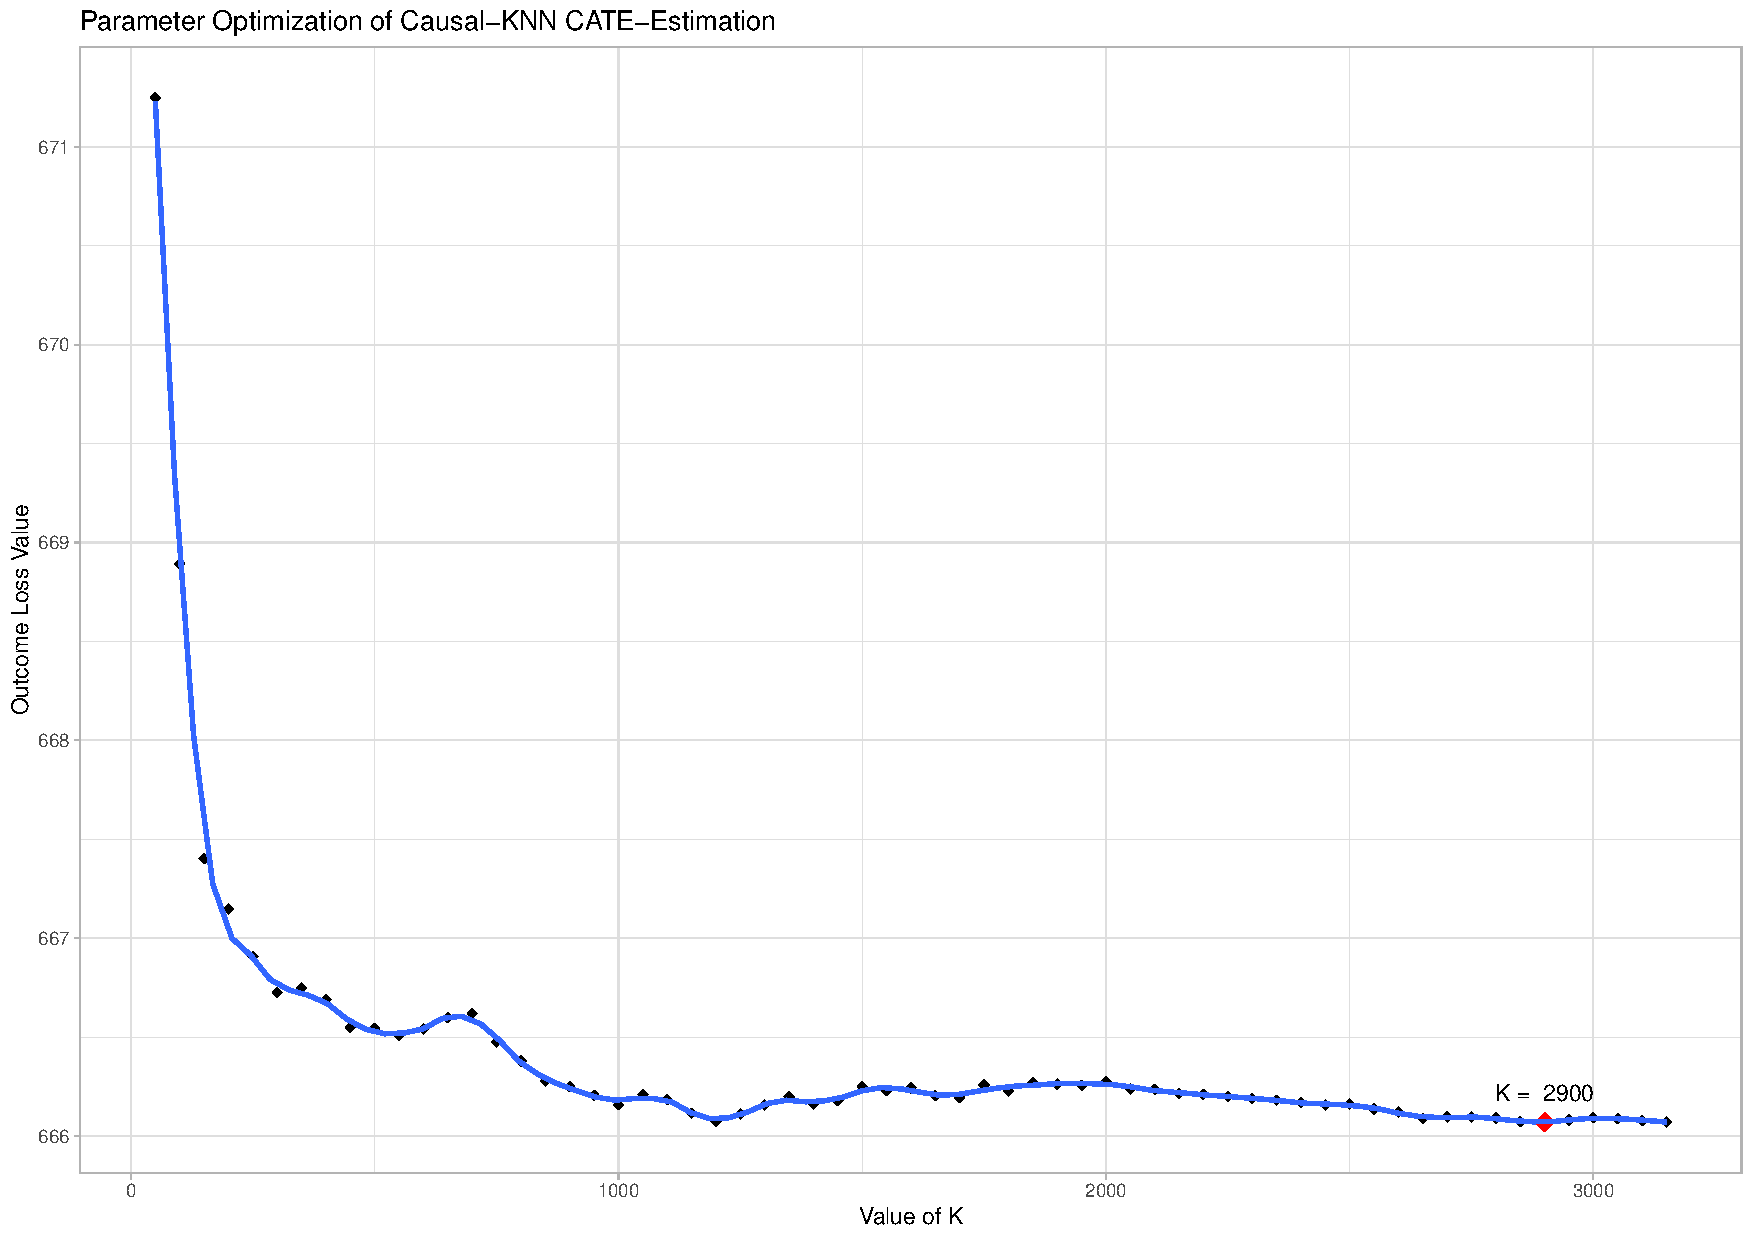
\includegraphics[width=10cm]{Objects/param_tuning_spend.pdf}
}

\frame{
\frametitle{Application: Results}
Outcome Variable: Spend (numeric) in \$ (US)
\begin{itemize}
\item ATE = 0.31321
\item ATT = 0.31205
\end{itemize}
\vspace{0.2cm}
\centering{
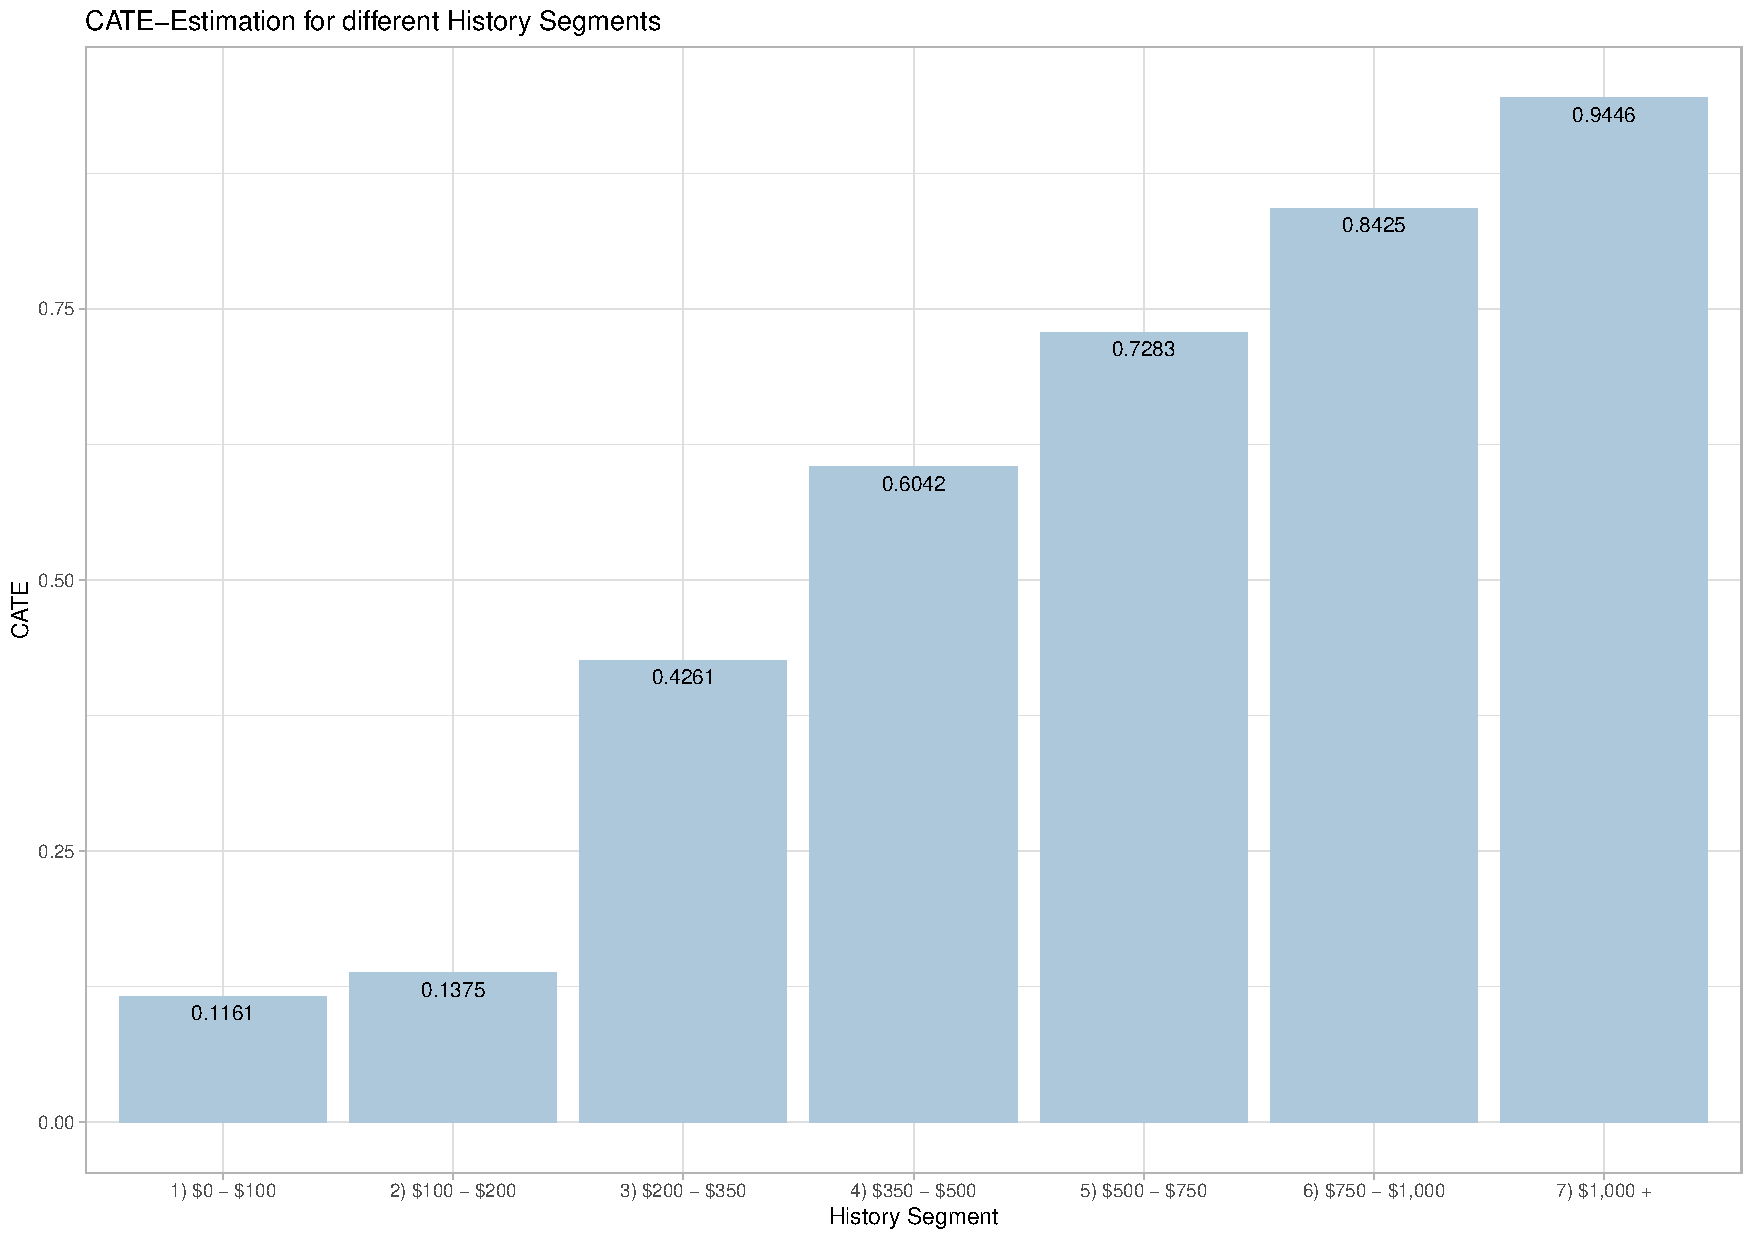
\includegraphics[width=7cm]{Objects/hist_seg_spend.pdf} \hspace{0.2cm}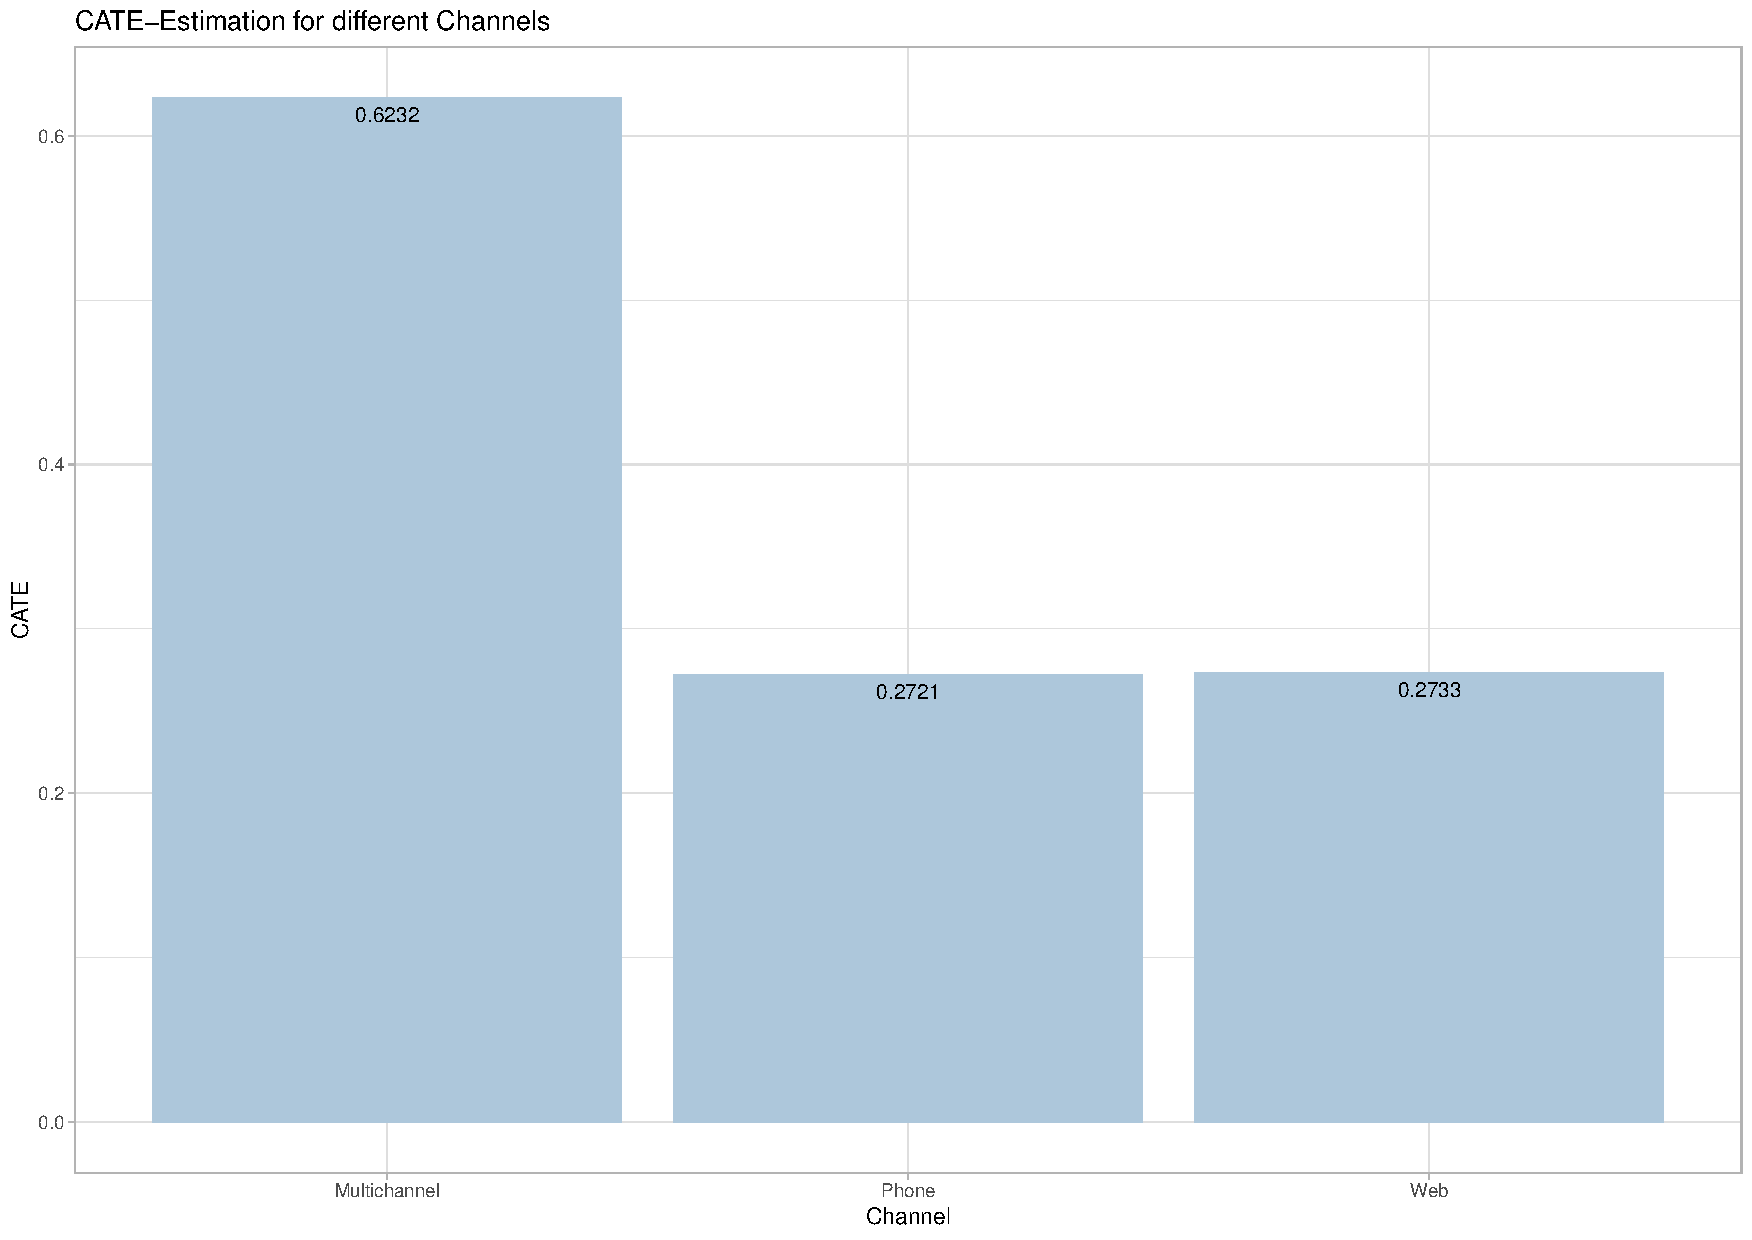
\includegraphics[width=7cm]{Objects/channel_spend.pdf}
}

%\vspace{0.1cm}
%\centering{
%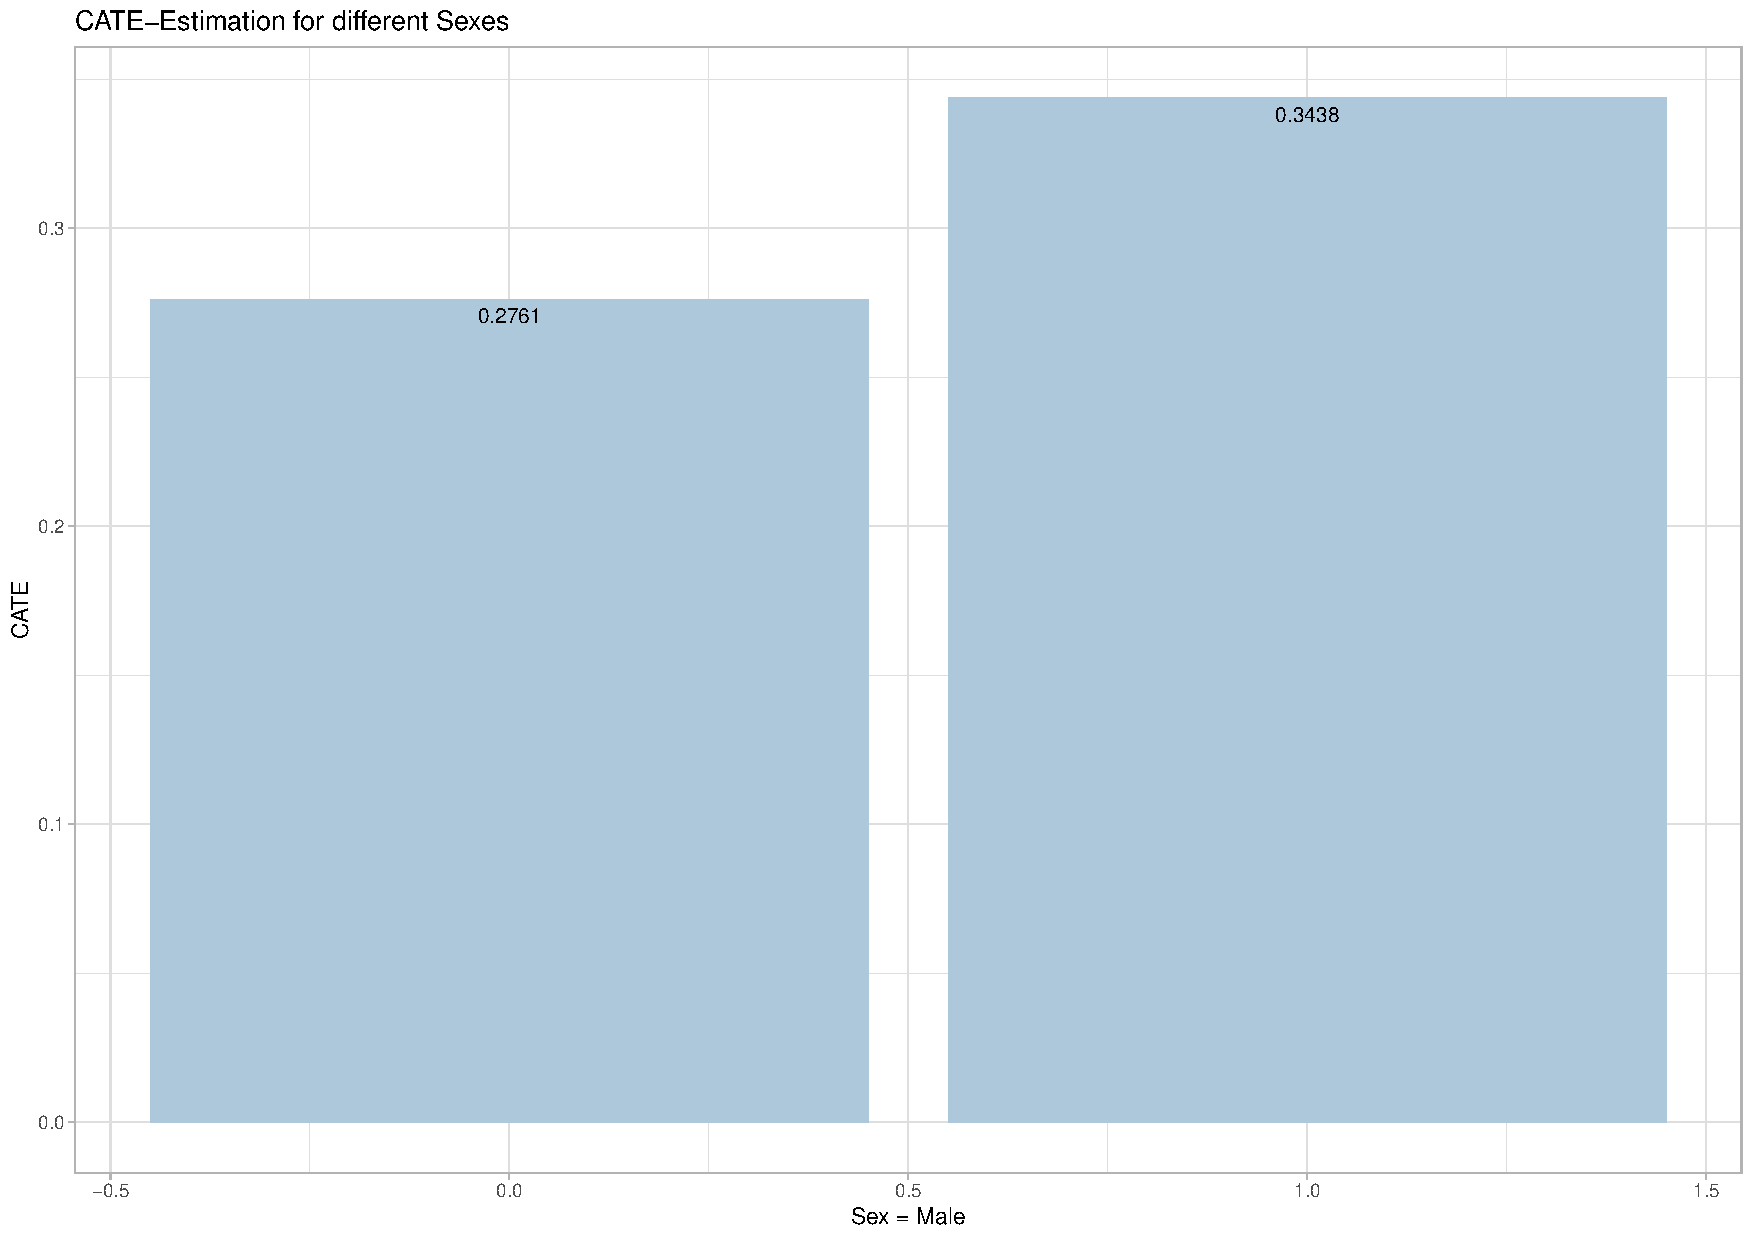
\includegraphics[width=4cm]{Objects/sex_spend.pdf} \hspace{1cm}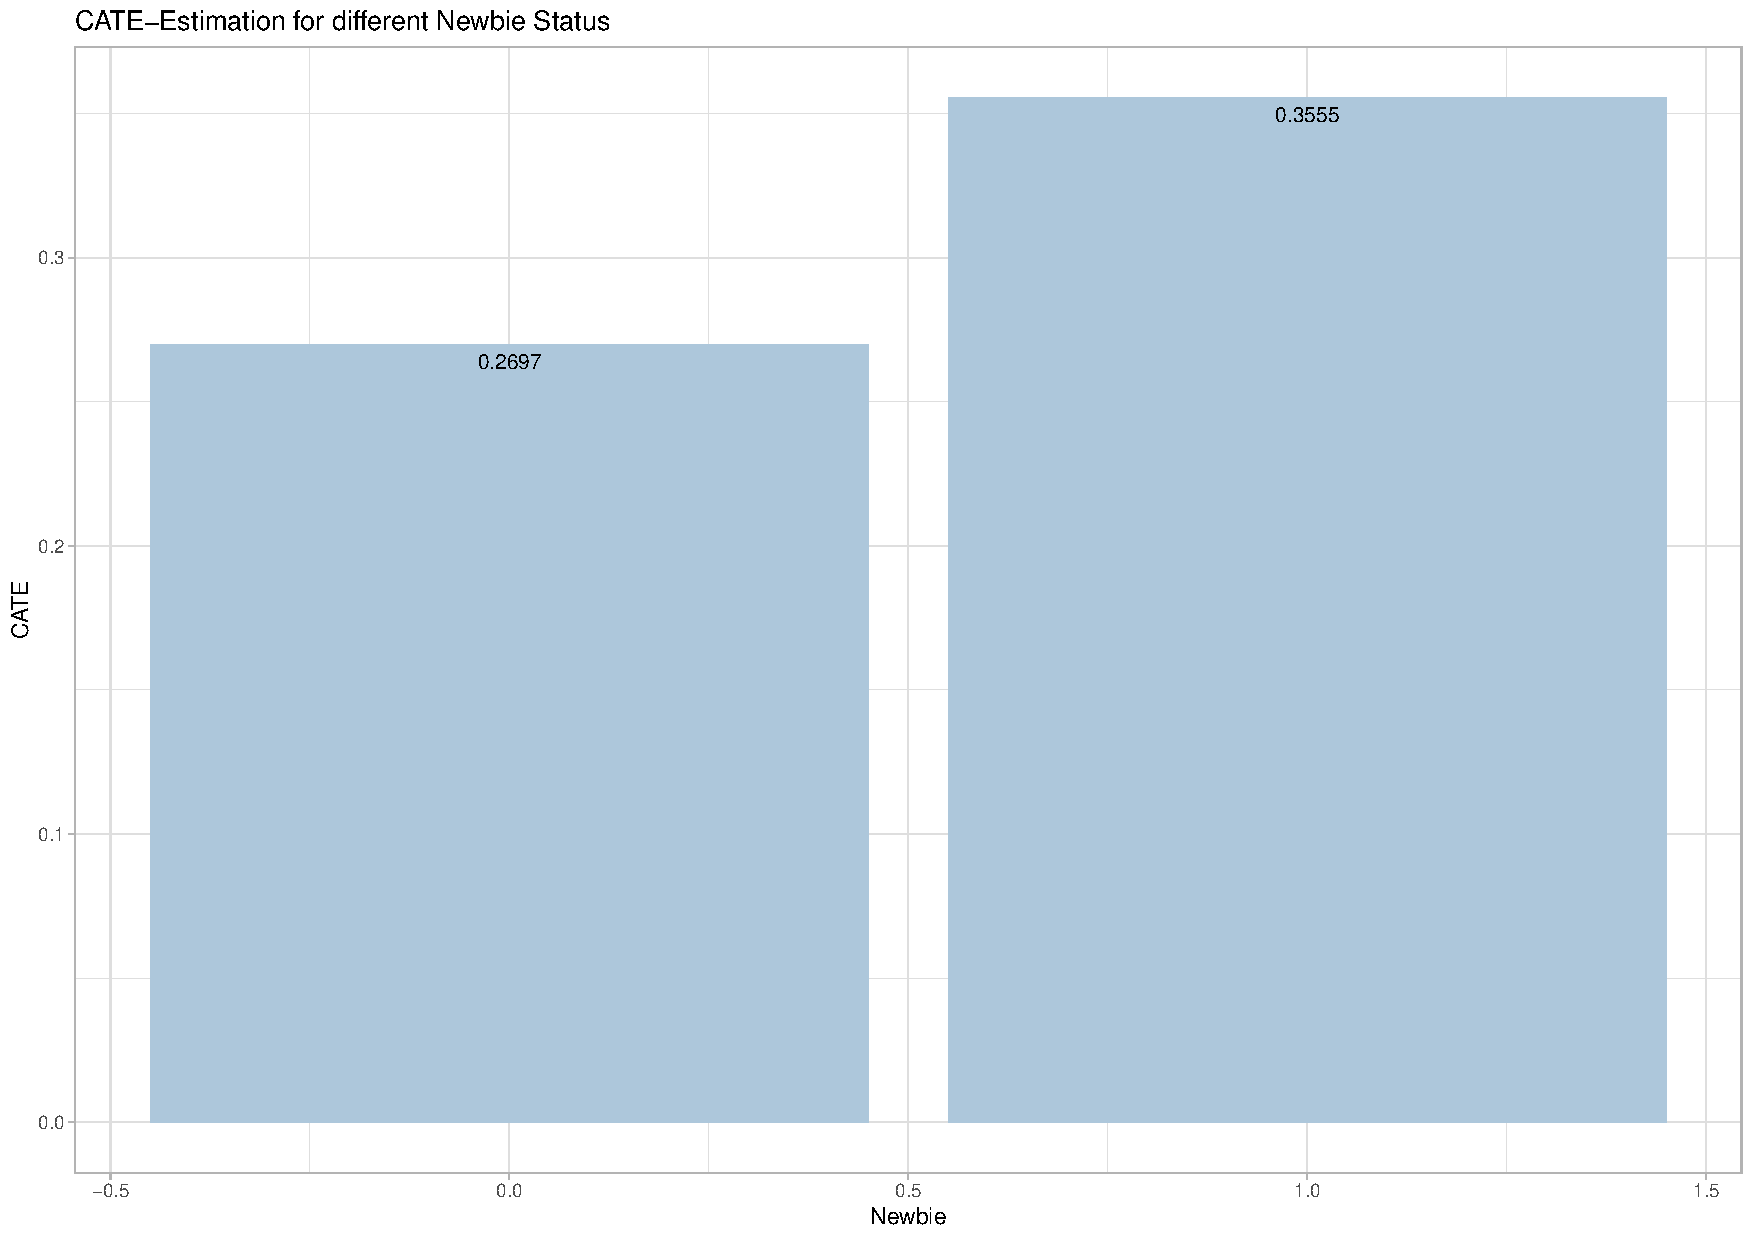
\includegraphics[width=4cm]{Objects/newbie_spend.pdf}
%}
}

\end{document}
